\documentclass[a4paper,12pt,twoside]{memoir}

% Castellano
\usepackage[spanish,es-tabla]{babel}
\selectlanguage{spanish}
\usepackage[utf8]{inputenc}
\usepackage[T1]{fontenc}
\usepackage{lmodern} % scalable font
\usepackage{microtype}
\usepackage{placeins}

\RequirePackage{booktabs}
\RequirePackage[table]{xcolor}
\RequirePackage{xtab}
\RequirePackage{multirow}

% Links
\PassOptionsToPackage{hyphens}{url}\usepackage[colorlinks]{hyperref}
\hypersetup{
	allcolors = {blue}
}

% Ecuaciones
\usepackage{amsmath}

% Rutas de fichero / paquete
\newcommand{\ruta}[1]{{\sffamily #1}}

% Párrafos
\nonzeroparskip

% Huérfanas y viudas
\widowpenalty100000
\clubpenalty100000

% Evitar solapes en el header
\nouppercaseheads

% Imagenes
\usepackage{graphicx}
\newcommand{\imagen}[2]{
	\begin{figure}[!h]
		\centering
		\includegraphics[width=0.9\textwidth]{#1}
		\caption{#2}\label{fig:#1}
	\end{figure}
	\FloatBarrier
}

\newcommand{\imagenflotante}[2]{
	\begin{figure}%[!h]
		\centering
		\includegraphics[width=0.9\textwidth]{#1}
		\caption{#2}\label{fig:#1}
	\end{figure}
}



% El comando \figura nos permite insertar figuras comodamente, y utilizando
% siempre el mismo formato. Los parametros son:
% 1 -> Porcentaje del ancho de página que ocupará la figura (de 0 a 1)
% 2 --> Fichero de la imagen
% 3 --> Texto a pie de imagen
% 4 --> Etiqueta (label) para referencias
% 5 --> Opciones que queramos pasarle al \includegraphics
% 6 --> Opciones de posicionamiento a pasarle a \begin{figure}
\newcommand{\figuraConPosicion}[6]{%
  \setlength{\anchoFloat}{#1\textwidth}%
  \addtolength{\anchoFloat}{-4\fboxsep}%
  \setlength{\anchoFigura}{\anchoFloat}%
  \begin{figure}[#6]
    \begin{center}%
      \Ovalbox{%
        \begin{minipage}{\anchoFloat}%
          \begin{center}%
            \includegraphics[width=\anchoFigura,#5]{#2}%
            \caption{#3}%
            \label{#4}%
          \end{center}%
        \end{minipage}
      }%
    \end{center}%
  \end{figure}%
}

%
% Comando para incluir imágenes en formato apaisado (sin marco).
\newcommand{\figuraApaisadaSinMarco}[5]{%
  \begin{figure}%
    \begin{center}%
    \includegraphics[angle=90,height=#1\textheight,#5]{#2}%
    \caption{#3}%
    \label{#4}%
    \end{center}%
  \end{figure}%
}
% Para las tablas
\newcommand{\otoprule}{\midrule [\heavyrulewidth]}
%
% Nuevo comando para tablas pequeñas (menos de una página).
\newcommand{\tablaSmall}[5]{%
 \begin{table}
  \begin{center}
   \rowcolors {2}{gray!35}{}
   \begin{tabular}{#2}
    \toprule
    #4
    \otoprule
    #5
    \bottomrule
   \end{tabular}
   \caption{#1}
   \label{tabla:#3}
  \end{center}
 \end{table}
}

%
%Para el float H de tablaSmallSinColores
\usepackage{float}

%
% Nuevo comando para tablas pequeñas (menos de una página).
\newcommand{\tablaSmallSinColores}[5]{%
 \begin{table}[H]
  \begin{center}
   \begin{tabular}{#2}
    \toprule
    #4
    \otoprule
    #5
    \bottomrule
   \end{tabular}
   \caption{#1}
   \label{tabla:#3}
  \end{center}
 \end{table}
}

\newcommand{\tablaApaisadaSmall}[5]{%
\begin{landscape}
  \begin{table}
   \begin{center}
    \rowcolors {2}{gray!35}{}
    \begin{tabular}{#2}
     \toprule
     #4
     \otoprule
     #5
     \bottomrule
    \end{tabular}
    \caption{#1}
    \label{tabla:#3}
   \end{center}
  \end{table}
\end{landscape}
}

%
% Nuevo comando para tablas grandes con cabecera y filas alternas coloreadas en gris.
\newcommand{\tabla}[6]{%
  \begin{center}
    \tablefirsthead{
      \toprule
      #5
      \otoprule
    }
    \tablehead{
      \multicolumn{#3}{l}{\small\sl continúa desde la página anterior}\\
      \toprule
      #5
      \otoprule
    }
    \tabletail{
      \hline
      \multicolumn{#3}{r}{\small\sl continúa en la página siguiente}\\
    }
    \tablelasttail{
      \hline
    }
    \bottomcaption{#1}
    \rowcolors {2}{gray!35}{}
    \begin{xtabular}{#2}
      #6
      \bottomrule
    \end{xtabular}
    \label{tabla:#4}
  \end{center}
}

%
% Nuevo comando para tablas grandes con cabecera.
\newcommand{\tablaSinColores}[6]{%
  \begin{center}
    \tablefirsthead{
      \toprule
      #5
      \otoprule
    }
    \tablehead{
      \multicolumn{#3}{l}{\small\sl continúa desde la página anterior}\\
      \toprule
      #5
      \otoprule
    }
    \tabletail{
      \hline
      \multicolumn{#3}{r}{\small\sl continúa en la página siguiente}\\
    }
    \tablelasttail{
      \hline
    }
    \bottomcaption{#1}
    \begin{xtabular}{#2}
      #6
      \bottomrule
    \end{xtabular}
    \label{tabla:#4}
  \end{center}
}

%
% Nuevo comando para tablas grandes sin cabecera.
\newcommand{\tablaSinCabecera}[5]{%
  \begin{center}
    \tablefirsthead{
      \toprule
    }
    \tablehead{
      \multicolumn{#3}{l}{\small\sl continúa desde la página anterior}\\
      \hline
    }
    \tabletail{
      \hline
      \multicolumn{#3}{r}{\small\sl continúa en la página siguiente}\\
    }
    \tablelasttail{
      \hline
    }
    \bottomcaption{#1}
  \begin{xtabular}{#2}
    #5
   \bottomrule
  \end{xtabular}
  \label{tabla:#4}
  \end{center}
}



\definecolor{cgoLight}{HTML}{EEEEEE}
\definecolor{cgoExtralight}{HTML}{FFFFFF}

%
% Nuevo comando para tablas grandes sin cabecera.
\newcommand{\tablaSinCabeceraConBandas}[5]{%
  \begin{center}
    \tablefirsthead{
      \toprule
    }
    \tablehead{
      \multicolumn{#3}{l}{\small\sl continúa desde la página anterior}\\
      \hline
    }
    \tabletail{
      \hline
      \multicolumn{#3}{r}{\small\sl continúa en la página siguiente}\\
    }
    \tablelasttail{
      \hline
    }
    \bottomcaption{#1}
    \rowcolors[]{1}{cgoExtralight}{cgoLight}

  \begin{xtabular}{#2}
    #5
   \bottomrule
  \end{xtabular}
  \label{tabla:#4}
  \end{center}
}




\graphicspath{ {./img/} }

% Capítulos
\chapterstyle{bianchi}
\newcommand{\capitulo}[2]{
	\setcounter{chapter}{#1}
	\setcounter{section}{0}
	\chapter*{#2}
	\addcontentsline{toc}{chapter}{#2}
	\markboth{#2}{#2}
}

% Apéndices
\renewcommand{\appendixname}{Apéndice}
\renewcommand*\cftappendixname{\appendixname}

\newcommand{\apendice}[1]{
	%\renewcommand{\thechapter}{A}
	\chapter{#1}
}

\renewcommand*\cftappendixname{\appendixname\ }

% Formato de portada
\makeatletter
\usepackage{xcolor}
\newcommand{\tutor}[1]{\def\@tutor{#1}}
\newcommand{\tutorEmp}[1]{\def\@tutorEmp{#1}}
\newcommand{\course}[1]{\def\@course{#1}}
\definecolor{cpardoBox}{HTML}{E6E6FF}
\def\maketitle{
  \null
  \thispagestyle{empty}
  % Cabecera ----------------
\noindent
\includegraphics[width=\textwidth]{cabecera}\vspace{1cm}%
  \vfill
  % Título proyecto y escudo informática ----------------
  \colorbox{cpardoBox}{%
    \begin{minipage}{.8\textwidth}
      \vspace{.5cm}\Large
      \begin{center}
      \textbf{TFG del Grado en Ingeniería Informática}\vspace{.6cm}\\
      \textbf{\LARGE\@title{}}
      \end{center}
      \vspace{.2cm}
    \end{minipage}

  }%
  \hfill\begin{minipage}{.20\textwidth}
    
\includegraphics[width=\textwidth]{escudoInfor}
  \end{minipage}
  \vfill
  % Datos de alumno, curso y tutores ------------------
  \begin{center}%
  {%
    \noindent\LARGE
    Presentado por \@author{}\\ 
    en la Universidad de Burgos --- 14 de junio de 2021{}\\
    Tutores académicos: \@tutor{} y  Nuño Basurto Hornillos\\
    Tutor empresarial (ITCL): \@tutorEmp{}\\
  }%
  \end{center}%
  \null
  \cleardoublepage
  }
\makeatother


% Datos de portada
\title{Asistente remoto en realidad aumentada y mixta con HoloLens 2 \\Documentación Técnica}
\author{Miguel Martín Valdivielso}
\tutor{Ángel Arroyo Puente}
\tutorEmp{Alejandro Langarica Aparicio}
\date{\today}

\begin{document}

\maketitle



\cleardoublepage



%%%%%%%%%%%%%%%%%%%%%%%%%%%%%%%%%%%%%%%%%%%%%%%%%%%%%%%%%%%%%%%%%%%%%%%%%%%%%%%%%%%%%%%%



\frontmatter


\clearpage

% Indices
\tableofcontents

\clearpage

\listoffigures

\clearpage

\listoftables

\clearpage

\mainmatter

\appendix

\apendice{Plan de Proyecto software}

\section{Introducción}

La planificación es fundamental durante el comienzo de un proyecto. En esta fase se realiza una estimación del trabajo, tiempo y recursos económicos que va a ser necesarios para la ejecución del proyecto. Esta planificación se divide en planificación temporal y estudio de viabilidad.

En la planificación temporal se comenzará marcando los objetivos técnicos y funcionales que componen el proyecto. Una vez establecidos estos objetivos, se dividirán en distintas tareas de mayor sencillez que serán repartidas a lo largo de un calendario. Posteriormente se asignará una estimación de tiempo aproximada a cada tarea. Finalmente se marcará la fecha de inicio y la fecha de finalización estimada del proyecto.

El estudio de viabilidad se centrará en el apartado económico y legal del proyecto, donde analizaremos la legalidad y el presupuesto relacionado con este.

Las dos partes que componen el estudio de viabilidad son:
\begin{itemize}
    \item \textbf{Viabilidad económica:} estimación de beneficios y costes que implica la realización del proyecto.
    \item \textbf{Viabilidad legal:} análisis de todas las licencias de las herramientas utilizadas en el desarrollo del proyecto.
\end{itemize}
\section{Planificación temporal}

Todo el desarrollo del proyecto ha sido basado sobre la metodología ágil Scrum. Se han seguido las principales características de esta metodología, a excepción de algunas como, las reuniones diarias con el equipo, ya que al ser el trabajo de fin de grado los máximos participantes en el equipo de desarrollo son un estudiante, más la guía recibida por los tutores durante las reuniones.

Las 300 horas disponibles del TFG fueron divididas en 10 \textit{sprints} con una duración de 1 semana (de lunes a viernes) por cada \textit{sprint}. Hay un \textit{sprint} final dedicado a la documentación y entrega del TFG.

\subsection{\textit{Sprint} 0 (08/02/2021 - 14/02/2021)}
Primer \textit{sprint} que marcó el inicio del proyecto. El tutor de ITCL me recomendó utilizar esta semana para realizar una primera toma de contacto con Unity y con las HoloLens 2 para que posteriormente, pudiese realizar estimaciones aproximadas del tiempo que iba a costar realizar cada tarea del proyecto.

Más tarde, seleccioné todas las herramientas de las que iba hacer uso durante todo el trabajo.

Las tareas planificadas en esta semana fueron:
\begin{enumerate}
    \item Elección del repositorio.
    \item Elección de la herramienta para la gestión de proyectos.
    \item Elección de la herramienta para el control de versiones.
    \item Elección de la herramienta para la documentación.
    \item Elección del entorno de desarrollo (IDE).
    \item Toma de contacto con Unity.
    \item Toma de contacto con las HoloLens 2.
\end{enumerate}
\imagen{sprint0}{Se muestra un gráfico con el cierre las tareas de \textit{sprint} número 0}
\subsection{\textit{Sprint} 1 (15/02/2021 - 21/02/2021)}
En esta semana tuve mi primera reunión con el tutor del centro tecnológico ITCL, donde establecimos los objetivos del proyecto y organizamos las tareas principales en las que se iba a dividir el desarrollo. 

Posteriormente investigué e instalé todos los recursos que iba a necesitar para desarrollar la aplicación en el software de Unity.

Las tareas planificadas en esta semana fueron:
\begin{enumerate}
    \item Investigación de Mixed Reality Toolkit.
    \item Instalación de Visual Studio 2019.
    \item Instalación del SDK (\textit{software development kit)} de Windows 10.
    \item Instalación del emulador de HoloLens 2 para el ordenador.
\end{enumerate}
\imagen{sprint1}{Se muestra un gráfico con el cierre las tareas de \textit{sprint} número 1}
\subsection{\textit{Sprint} 2 (22/02/2021 - 28/02/2021)}
Los objetivos de este \textit{sprint} fueron: la configuración del proyecto de Unity y la instalación de los \textit{plugins} necesarios. Una vez configurado todo, se experimentará con los ejemplos proporcionados por el \textit{plugin} y se realizará una \textit{build} de prueba en las HoloLens 2. Al final de la semana iniciar la documentación con \LaTeX  usando el editor online Overleaf.

Las tareas planificadas en esta semana fueron:
\begin{enumerate}
    \item Configuración del proyecto.
    \item Instalación de Mixed Reality Toolkit.
    \item Aprendizaje de Mixed Reality Toolkit.
    \item \textit{Build} de prueba.
    \item Inicio de la documentación.
\end{enumerate}
\imagen{sprint2}{Se muestra un gráfico con el cierre las tareas de \textit{sprint} número 2}
\subsection{\textit{Sprint} 3 (01/03/2021 - 07/03/2021)} \label{spint3}
Una vez realizada una toma de contacto con Mixed Reality Toolkit la labor de esta semana consistirá en realizar uno de los objetivos principales del proyecto: Detectar el espacio real y generar objetos virtuales anclados a ese espacio.

Para lograr estos objetivos primero investigué la forma de obtener el objeto virtual correspondiente al espacio real. Una vez obtenido ese objeto realicé una \textit{build} de prueba, donde cada vez que realizaba un gesto con la mano generaba un objeto en realidad aumentada.

Las tareas planificadas en esta semana fueron:
\begin{enumerate}
    \item Obtener la asignación espacial.
    \item Lanzar un \textit{raycast} y que colisione con la asignación espacial.
    \item Generar un objeto en las coordenadas de la colisión.
    \item Realizar \textit{build} para probar las funcionalidades implementadas.
    \item Ampliar documentación.
\end{enumerate}
\imagen{sprint3}{Se muestra un gráfico con el cierre las tareas de \textit{sprint} número 3}
\subsection{\textit{Sprint} 4 (08/03/2021 - 14/03/2021)}
Una vez cumplidas las tareas del \textit{sprint} anterior se investigará como conectar la aplicación de las HoloLens 2 con un ordenador. Esta semana estuvo dedicada completamente a probar diferentes métodos y herramientas que cumplieses con las necesidades de mi proyecto.

La conclusión sacada esta semana sobre la herramienta a utilizar fue el proyecto de código abierto WebRTC. 

Las tareas planificadas en esta semana fueron:
\begin{enumerate}
    \item Investigar cómo realizar la conexión entre las 2 aplicaciones.
    \item Prueba de Photon Unity Network 2.
    \item Prueba de Microsoft Azure.
    \item Prueba de WebRTC.
\end{enumerate}
\imagen{sprint4}{Se muestra un gráfico con el cierre las tareas de \textit{sprint} número 4}
\subsection{\textit{Sprint} 5 (15/03/2021 - 21/03/2021)} \label{spint5}
Los objetivos de este \textit{sprint} fueron: aprender a usar WebRTC para desarrollar 2 aplicaciones que se puedan comunicar compartiendo vídeo en tiempo real entre ambas y realizar un prototipo de videollamada.

Durante esta semana surgieron numerosos \textit{bugs} relacionados con la configuración de WebRTC y la comunicación de la señal de video. El prototipo de videollamada realizado al final de la semana también tuvo un gran número problemas relacionados con el rendimiento de la aplicación de las HoloLens 2.

Las tareas planificadas en esta semana fueron:
\begin{enumerate}
    \item Instalación del proyecto node-dss.
    \item Configurar el proyecto de Unity con el \textit{raycast} de WebRTC.
    \item Detectar la \textit{webcam} del ordenador.
    \item Detectar la cámara de las HoloLens 2.
    \item Compartir la señal de video entre las aplicaciones.
    \item Crear un prototipo de videollamada.
\end{enumerate}
En este \textit{sprint} cerré todas las tareas al final de la semana por eso el gráfico tiene esta forma (véase Fig A.3 sección \ref{fig1}).
\imagen{sprint5}{Se muestra un gráfico con el cierre las tareas de \textit{sprint} número 5} \label{fig1}
\subsection{\textit{Sprint} 6 (22/03/2021 - 28/03/2021)}
Los objetivos de este \textit{sprint} fueron:
\begin{enumerate}
    \item Arreglar el \textit{bug} de rendimiento de la semana anterior.
    \item Juntar los prototipos creados en: el \textit{sprint} 3 y 5.
    \item Enviar las coordenadas a las HoloLens 2 haciendo clic en la pantalla.
    \item Recibir las coordenadas.
    \item Generar el objeto en realidad mixta.
    \item Hacer \textit{build} y probar todas las funcionalidades implementadas.
\end{enumerate}

Esta semana fue la que mayor carga de trabajo tuvo debido al gran número de funcionalidades a pensar e implementar. A esto se le suman los problemas que surgieron para calibrar la generación del objeto virtual.

Las tareas planificadas en esta semana fueron:
\begin{enumerate}
    \item Juntar la videollamada con la asignación espacial.
    \item Comprobar que todo funcione correctamente.
    \item Enviar mensajes desde el ordenador.
    \item Recibir mensajes en las HoloLens 2.
    \item A través de las coordenadas recibidas lanzar un \textit{raycast}.
    \item Generar un objeto donde colisione un \textit{raycast} con la asignación espacial.
    \item Hacer \textit{build} de las dos aplicaciones para probar las funcionalidades implementadas.
\end{enumerate}
Al igual que en la semana anterior cerré todas las tareas al final de la semana por eso el gráfico tiene esta forma (véase Fig A.5 sección \ref{fig3}).
\imagen{sprint6}{Se muestra un gráfico con el cierre las tareas de \textit{sprint} número 6}\label{fig3}
\subsection{\textit{Sprint} 7 (29/03/2021 - 04/04/2021)}
Los objetivos de este \textit{sprint} fueron: implementar funcionalidades características de una video llamada y diseñar una interfaz para las HoloLens 2 para así poder acceder a esas funcionalidades.

Tras implementar todas las funcionalidades volvió a aparecer el \textit{bug} de rendimiento del sprint 5.

Las tareas planificadas en esta semana fueron:
\begin{enumerate}
    \item Pensar las funcionalidades a implementar.
    \item Crear una barra de menú.
    \item Implementar seguimiento radial al menú.
    \item Permitir que el menú sea manipulable.
    \item Crear botón de colgar.
    \item Crear botón de silenciar el micrófono.
    \item Crear botón de esconder la \textit{webcam}.
    \item Crear botón de ensordecer la llamada.
    \item Crear botón de esconder la interfaz.
    \item Probar los cambios.
    
\end{enumerate}
\imagen{sprint7}{Se muestra un gráfico con el cierre las tareas de \textit{sprint} número 7}
\subsection{\textit{Sprint} 8 (05/04/2021 - 11/04/2021)}
Los objetivos de este \textit{sprint} fueron: implementar las funcionalidades características de una video llamada y diseñar una interfaz en la aplicación del ordenador para acceder a estas.

Las tareas planificadas en esta semana fueron:
\begin{enumerate}
    \item Crear una barra de menú.
    \item Crear botón de generar flechas.
    \item Crear botón de borrar todas las flechas.
    \item Crear botón de borrar la última flecha generada
    \item Crear botón de colgar.
    \item Crear botón de silenciar el micrófono.
    \item Crear botón de esconder la \textit{webcam}.
\end{enumerate}
\imagen{sprint8}{Se muestra un gráfico con el cierre las tareas de \textit{sprint} número 8}
\subsection{\textit{Sprint} 9 (12/04/2021 - 18/04/2021)}
Los objetivos de este \textit{sprint} fueron: arreglar los \textit{bugs} arrastrados de otros \textit{sprints}, pulir lo máximo posible los prototipos y lanzar las versiones finales de las aplicaciones.

Las tareas planificadas en esta semana fueron:
\begin{enumerate}
    \item Arreglar \textit{bug} rendimiento.
    \item Arreglar \textit{bug} del sonido duplicado. 
    \item Organizar escena de Unity. 
    \item Realizar la \textit{build} final.
\end{enumerate}
\imagen{sprint9}{Se muestra un gráfico con el cierre las tareas de \textit{sprint} número 9}
\subsection{\textit{Sprint} 10 (19/04/2021 - Activo)}
Este último \textit{sprint} está dedicado a la finalización de la documentación y a preparar la entrega del TFG el 14 de Junio de 2021.

Las tareas planificadas en \textit{sprint} fueron:
\begin{enumerate}
    \item Finalizar la documentación.
    \item Realizar entrega del todos los materiales relacionado con el TFG.
\end{enumerate}
Por último, se mostrará la evolución de las tareas a lo largo del tiempo (véase Fig A.11 sección \ref{fig2}) y la carga de trabajo de los \textit{sprints} (véase Fig A.12 sección \ref{fig4}).
\imagen{issues}{Se muestra un gráfico con el despliegue en el tiempo las tareas realizadas}\label{fig2}
\imagen{issues2}{Se muestra un gráfico con la carga de trabajo de los 7 últimos \textit{sprints} del proyecto}\label{fig4}
\section{Estudio de viabilidad}
\subsection{Viabilidad económica}

En esta sección analizaremos los costes económicos para poder llevar a cabo el desarrollo del proyecto en un entorno real.

\subsubsection{Costes de personal}

El proyecto se ha llevado a cabo por un único desarrollador durante 10 semanas con una jornada laboral de 6 horas al día. Considerando un salario bruto de 20000€ anuales, el coste del personal sería el siguiente:

\tablaSmallSinColores{Coste del personal}{ l | c }{coste_personal}
{\textbf{Concepto} & \textbf{Coste} \\}{
    Salario mensual neto & 1.366,0€ \\
    Retención del IRPF & 194,83€ \\
    Cuotas a la Seg. Social  & 471,66€ \\
    Coste mensual del trabajador & 2.032,49€ \\ \hline
    \textbf{Coste total de las 10 semanas} & 5.081,22€ \\
}
La cuota a la seguridad social es del 28,3\% \cite{ss:porcentaje} y la retención del IRPF es del 11,69\% \cite{hacienda:somostodos}.



\subsubsection{Costes de hardware}

En este apartado añadiremos todos los costes relacionados a dispositivos hardware utilizados en el proyecto. Consideramos una amortización a los 5 años y un uso de 2 meses y medio.

\tablaSmallSinColores{Coste del hardware}{ l | c | c }{coste_hardware}
{\textbf{Concepto}\hspace{0.5cm} & \hspace{0.5cm}\textbf{Coste}\hspace{0.5cm} & \hspace{0.5cm}\textbf{Amortización} \\}{
    Ordenador & 500€ & 104,17€\\
    HoloLens 2 & 3.849€ & 801,90€\\ \midrule
    \textbf{Total} & 4.349€ & 906,07€\\ 
}El precio del ordenador está basado en una aproximación que tiene en cuenta el valor de los componentes que marcan los requisitos recomendados por Unity.

\subsubsection{Costes de software} \label{software}

En este apartado añadiremos todos los costes relacionados a licencias de software utilizadas en el proyecto. Consideramos una amortización de 2 años.

\tablaSmallSinColores{Coste del hardware}{ l | c | c }{coste_software}
{\textbf{Concepto}\hspace{0.5cm} & \hspace{0.5cm}\textbf{Coste}\hspace{0.5cm} & \hspace{0.5cm}\textbf{Amortización} \\}{
    Windows 10 Home & 145€ & 54,37€\\ \hline
    \textbf{Total} & 145€ & 54,37€\\ 
}

En un supuesto en el que se comercializase la aplicación y esta generase un beneficio mayor de 100000 dólares, sería necesario comprar la licencia de Unity Pro que tiene un valor de 150 dólares mensuales.

\subsubsection{Costes totales}
La suma de los costes totales es la siguiente:

\tablaSmallSinColores{Coste total}{ l | c }{coste_total}
{\textbf{Concepto} & \textbf{Coste} \\}{
    Personal & 5.081,22€ \\
    Hardware & 906,07€ \\
    Software  & 54,37€ \\ \hline
    \textbf{Coste total} & 6.041,66€ \\
}

\subsection{Viabilidad legal}
 En este apartado se mostrará las licencias de todo el software involucrado en la creación del proyecto.
 
\tablaSmallSinColores{Licencias}{ l | l }{licencias}
{\textbf{software} & \textbf{Licencia} \\}{
    Mixed Reality ToolKit & MIT License \\
    WebRTC for Mixed Reality & MIT License\\
    Node-dss & MIT License\\
    Node.js  & MIT License\\ \hline
    Documentación & CC-BY-4.0 \\
}

Haciendo alusión al apartado de los costes de software \ref{software}, en un principio no sería necesario pagar la versión Pro de Unity si no superamos los 100000 dólares de beneficio. Por lo tanto, no tendríamos ningún problema para comercializar el software.

En este proyecto se ha hecho uso de programas opcionales como Rider y GitKraken, cuyas licencias venían incluidas en el GitHub Student Developer Pack al que se tienen acceso por ser estudiante de la Universidad de Burgos. En un entorno empresarial real sería necesario adquirir ambas licencias para hacer uso de este software.

\subsection{Licencia final del producto}

Todos los materiales entregados en este TFG contarán con una licencia BY-NC-SA 4.0. Esta licencia permite el uso para fines académicos no comerciales. Se permite cualquier modificación mientras se siga manteniendo la misma licencia y la condición de mencionar al autor original.

Al ser un prototipo realizado para ITCL, en el momento que este pase a ser un proyecto real, la licencia comercial del producto final podrá variar en consideración de ITCL.
\apendice{Especificación de Requisitos}

\section{Introducción}
En esta sección documentaremos las funcionalidades y el alcance que va a tener el proyecto. Se mostrará en detalle los objetivos generales de la aplicación, los requisitos funcionales y los casos de uso.
\section{Objetivos generales}
El objetivo general es desarrollar una aplicación de escritorio para un ordenador con Windows y HoloLens 2 que permita:
\begin{enumerate}
    \item Iniciar la llamada.
    \item Compartir señal de vídeo.
    \item Compartir señal de audio.
    \item Asistencia remota.
    \item Interfaz para acceder a las funciones de la videoconferencia.
    \item Manipular la interfaz.
    \item Finalizar llamada.
\end{enumerate}

\section{Catálogo de requisitos}

\subsection{Requisitos funcionales}
\begin{itemize}
\tightlist
\item
    \textbf{RF-1:} Iniciar la videoconferencia.
    
    \begin{itemize}
    \tightlist
    \item
        \textbf{RF-1.1:} Generar un código desde las HoloLens 2.
    \item
        \textbf{RF-1.2:} Introducir código en el ordenador para iniciar la llamada.
        \begin{itemize}
        \tightlist
        \item
            \textbf{RF-1.2.1:} Botón de iniciar la llamada.
        \end{itemize}
    \end{itemize}
\item
    \textbf{RF-2:} Usar la videoconferencia.
    \begin{itemize}
    \tightlist
    \item
        \textbf{RF-2.1:} Visualizar la perspectiva de las HoloLens 2 desde el ordenador.
        \begin{itemize}
        \tightlist
        \item
            \textbf{RF-2.1.1:} Recibir señal de vídeo en el ordenador.
        \item
            \textbf{RF-2.1.2:} Recibir señal de audio en el ordenador.
        \end{itemize}
    \item
        \textbf{RF-2.2:} Interfaz de la aplicación del ordenador.
        \begin{itemize}
        \tightlist
        \item
            \textbf{RF-2.2.1:} Botón para generar indicadores.
        \item
            \textbf{RF-2.2.2:} Botón para deshacer el último indicador generado.
        \item
            \textbf{RF-2.2.3:} Botón para borrar todos los indicadores.
        \item
            \textbf{RF-2.2.4:} Botón para silenciar el micrófono.
        \item
            \textbf{RF-2.2.5:} Botón para apagar la \textit{webcam}.
        \end{itemize}
    \item
        \textbf{RF-2.3:} Comunicación con otro usuario desde las HoloLens 2.
        \begin{itemize}
        \tightlist
        \item
            \textbf{RF-2.3.1:} Recibir señal de vídeo en las HoloLens 2.
        \item
            \textbf{RF-2.3.2:} Recibir señal de audio en las HoloLens 2.
        \end{itemize}
    \item
        \textbf{RF-2.4:} Interfaz de la aplicación de las HoloLens 2.
        \begin{itemize}
        \tightlist
        \item
            \textbf{RF-2.4.1:} Botón para silenciar el micrófono.
        \item
            \textbf{RF-2.4.2:} Botón para apagar la \textit{webcam}.
        \item
            \textbf{RF-2.4.3:} Botón de ensordecer.
        \item
            \textbf{RF-2.4.4:} Botón del seguimiento radial de la interfaz.
        \item
            \textbf{RF-2.4.5:} Botón para ocultar la interfaz.
        \end{itemize}
    \item
        \textbf{RF-2.5:} Manipular la interfaz de las HoloLens 2.
    \item
        \textbf{RF-2.6:} Asistencia Remota.
        \begin{itemize}
        \tightlist
        \item
            \textbf{RF-2.6.1:} Enviar coordenadas desde el ordenador.
        \item
            \textbf{RF-2.6.2:} Recibir coordenadas en las HoloLens 2 y generar el indicador.
        \end{itemize}
    \end{itemize}
    
\item
    \textbf{RF-3:} Finalizar la videoconferencia.
    \begin{itemize}
    \tightlist
    \item
    \textbf{RF-3.1:} Botón de finalizar llamada.
    \item
    \textbf{RF-3.2:} Vuelta a la pantalla de inicio.
    \end{itemize}
\end{itemize}

\subsection{Requisitos no funcionales}
\begin{itemize}
    \item \textbf{RNF-1 Escalabilidad:} Este requisito es el más importante debido a que al ser un prototipo, este debe poder ser escalable ya que en un futuro la empresa ITCL lo usará como la base de un nuevo proyecto.
    \item \textbf{RNF-2 Rendimiento:} En este tipo de aplicaciones relacionadas con la realidad virtual y aumentada el rendimiento es bastante importante, ya que cuanto más fluida sea la aplicación mejor experiencia proporcionará al usuario.
    \item \textbf{RNF-3 Comodidad:} Este requisito está directamente relacionado con el anterior, puesto que cuanto mayor rendimiento posea la aplicación mayor comodidad ofrecerá al usuario, evitando así los posibles dolores de cabeza y mareos que son bastante frecuentes usando por primera vez estas tecnologías.
    \item \textbf{RNF-4 Mantenimiento:} La aplicación debe ser de fácil mantenimiento para poder ajustarse a su escalabilidad.
\end{itemize}


\subsection{Requisitos del cliente}  

El único requisito exigido por la empresa ITCL ha sido utilizar el software de Unity para el desarrollo del trabajo de fin de carrera. 

\section{Especificación de requisitos}

\begin{table}[ht!]
\centering
\begin{tabular}{|l|p{0.8\linewidth}|}
\hline
\multicolumn{2}{|l|}{\cellcolor[HTML]{C0C0C0}RF-1.1: Generar un código desde las HoloLens 2.}                                                           \\ \hline
Versión         & 1.0                                                                                                                                               \\ \hline
Autor           & Miguel Martín     \\ \hline
Descripción     & \begin{tabular}[c]{@{}p{\linewidth}@{}} La aplicación de las HoloLens 2 debe generar un código.\end{tabular} \\ \hline
Precondiciones  & Ninguna.  \\ \hline
Acciones        & El usuario abre la aplicación de las HoloLens 2.   \\ \hline
Postcondiciones & \begin{tabular}[c]{@{}p{\linewidth}@{}}El usuario comparte el código con el técnico que se encuentra en el ordenador.\end{tabular}                  \\ \hline
Excepciones     & \begin{tabular}[c]{@{}p{\linewidth}@{}}Ninguna.\end{tabular}                  \\ \hline
Importancia     & Alta                                                                                                                                          \\ \hline
\end{tabular}
\caption{RF-1.1:Generar un código desde las HoloLens 2.}
\end{table}

\begin{table}[ht!]
\centering
\begin{tabular}{|l|p{0.8\linewidth}|}
\hline
\multicolumn{2}{|l|}{\cellcolor[HTML]{C0C0C0}RF-1.2: Introducir código en el ordenador para iniciar la llamada.}                                                           \\ \hline
Versión         & 1.0                                                                                                                                               \\ \hline
Autor           & Miguel Martín     \\ \hline
Descripción     & \begin{tabular}[c]{@{}p{\linewidth}@{}}  El usuario debe introducir el código en la interfaz para poder iniciar la llamada.\end{tabular} \\ \hline
Precondiciones  & Recibir el código del otro usuario.  \\ \hline
Acciones        & El técnico introduce el código de las HoloLens 2.   \\ \hline
Postcondiciones & \begin{tabular}[c]{@{}p{\linewidth}@{}}Ninguna.\end{tabular}                  \\ \hline
Excepciones     & \begin{tabular}[c]{@{}p{\linewidth}@{}}Ninguna.\end{tabular}                  \\ \hline
Importancia     & Alta                                                                                                                                          \\ \hline
\end{tabular}
\caption{RF-1.2: Introducir código en el ordenador para iniciar la llamada.}
\end{table}


\begin{table}[ht!]
\centering
\begin{tabular}{|l|p{0.8\linewidth}|}
\hline
\multicolumn{2}{|l|}{\cellcolor[HTML]{C0C0C0}RF-1.2.1: Botón de iniciar la llamada.}                                                           \\ \hline
Versión         & 1.0                                                                                                                                               \\ \hline
Autor           & Miguel Martín     \\ \hline
Descripción     & \begin{tabular}[c]{@{}p{\linewidth}@{}} El técnico inicia la llamada tras pulsar el botón de la interfaz.\end{tabular} \\ \hline
Precondiciones  & Haber colocado el código en la interfaz.  \\ \hline
Acciones        & El técnico pulsa el botón.   \\ \hline
Postcondiciones & \begin{tabular}[c]{@{}p{\linewidth}@{}}Se inicia la videoconferencia entre las HoloLens 2 y el ordenador.\end{tabular}                  \\ \hline
Excepciones     & \begin{tabular}[c]{@{}p{\linewidth}@{}}Ninguna.\end{tabular}                  \\ \hline
Importancia     & Muy alta                                                                                                                                          \\ \hline
\end{tabular}
\caption{RF-1.2.1: Botón de iniciar la llamada..}
\end{table}


\begin{table}[ht!]
\centering
\begin{tabular}{|l|p{0.8\linewidth}|}
\hline
\multicolumn{2}{|l|}{\cellcolor[HTML]{C0C0C0}RF-2.1: Visualizar la perspectiva de las HoloLens 2 desde el ordenador.}                                                           \\ \hline
Versión         & 1.0                                                                                                                                               \\ \hline
Autor           & Miguel Martín     \\ \hline
Descripción     & \begin{tabular}[c]{@{}p{\linewidth}@{}} El técnico desde el ordenador debe ser capaz de ver la perspectiva de las HoloLens 2 y escuchar al usuario.\end{tabular} \\ \hline
Precondiciones  & Establecer la conexión.  \\ \hline
Acciones        & El técnico mira la pantalla y se coloca unos auriculares.   \\ \hline
Postcondiciones & \begin{tabular}[c]{@{}p{\linewidth}@{}}Ninguna.\end{tabular}                  \\ \hline
Excepciones     & \begin{tabular}[c]{@{}p{\linewidth}@{}}Ninguna.\end{tabular}                  \\ \hline
Importancia     & Muy alta                                                                                                                                          \\ \hline
\end{tabular}
\caption{RF-2.1: Visualizar la perspectiva de las HoloLens 2 desde el ordenador.}
\end{table}


\begin{table}[ht!]
\centering
\begin{tabular}{|l|p{0.8\linewidth}|}
\hline
\multicolumn{2}{|l|}{\cellcolor[HTML]{C0C0C0}RF-2.1.1: Recibir señal de vídeo en el ordenador.}                                                           \\ \hline
Versión         & 1.0                                                                                                                                               \\ \hline
Autor           & Miguel Martín     \\ \hline
Descripción     & \begin{tabular}[c]{@{}p{\linewidth}@{}} El técnico desde el ordenador debe ser capaz de ver la perspectiva de las HoloLens 2.\end{tabular} \\ \hline
Precondiciones  & Enviar el vídeo desde las HoloLens 2.  \\ \hline
Acciones        & El técnico ve la perspectiva del usuario.   \\ \hline
Postcondiciones & \begin{tabular}[c]{@{}p{\linewidth}@{}}Ninguna.\end{tabular}                  \\ \hline
Excepciones     & \begin{tabular}[c]{@{}p{\linewidth}@{}}Ninguna.\end{tabular}                  \\ \hline
Importancia     & Muy alta                                                                                                                                          \\ \hline
\end{tabular}
\caption{RF-2.1.1: Recibir señal de vídeo en el ordenador.}
\end{table}


\begin{table}[ht!]
\centering
\begin{tabular}{|l|p{0.8\linewidth}|}
\hline
\multicolumn{2}{|l|}{\cellcolor[HTML]{C0C0C0}RF-2.1.2: Recibir señal de audio en el ordenador.}                                                           \\ \hline
Versión         & 1.0                                                                                                                                               \\ \hline
Autor           & Miguel Martín     \\ \hline
Descripción     & \begin{tabular}[c]{@{}p{\linewidth}@{}} El técnico desde el ordenador debe ser capaz de escuchar al usuario con las HoloLens 2.\end{tabular} \\ \hline
Precondiciones  & Enviar el audio desde las HoloLens 2.  \\ \hline
Acciones        & El técnico escucha al usuario.   \\ \hline
Postcondiciones & \begin{tabular}[c]{@{}p{\linewidth}@{}}Ninguna.\end{tabular}                  \\ \hline
Excepciones     & \begin{tabular}[c]{@{}p{\linewidth}@{}}Ninguna.\end{tabular}                  \\ \hline
Importancia     & Muy alta                                                                                                                                          \\ \hline
\end{tabular}
\caption{RF-2.1.2: Recibir señal de audio en el ordenador.}
\end{table}


\begin{table}[ht!]
\centering
\begin{tabular}{|l|p{0.8\linewidth}|}
\hline
\multicolumn{2}{|l|}{\cellcolor[HTML]{C0C0C0}RF-2.2: Interfaz de la aplicación del ordenador.}                                                           \\ \hline
Versión         & 1.0                                                                                                                                               \\ \hline
Autor           & Miguel Martín     \\ \hline
Descripción     & \begin{tabular}[c]{@{}p{\linewidth}@{}} El técnico será capaz de utilizar todas las funcionalidades que ofrece la interfaz.\end{tabular} \\ \hline
Precondiciones  & Establecer la conexión.  \\ \hline
Acciones        & El técnico utiliza el ratón del ordenador para interactuar con la interfaz.   \\ \hline
Postcondiciones & \begin{tabular}[c]{@{}p{\linewidth}@{}}Se ejecuta la funcionalidad seleccionada.\end{tabular}                  \\ \hline
Excepciones     & \begin{tabular}[c]{@{}p{\linewidth}@{}}Ninguna.\end{tabular}                  \\ \hline
Importancia     & Alta                                                                                                                                          \\ \hline
\end{tabular}
\caption{RF-2.2: Interfaz de la aplicación del ordenador.}
\end{table}


\begin{table}[ht!]
\centering
\begin{tabular}{|l|p{0.8\linewidth}|}
\hline
\multicolumn{2}{|l|}{\cellcolor[HTML]{C0C0C0}RF-2.2.1: Botón para generar indicadores.}                                                           \\ \hline
Versión         & 1.0                                                                                                                                               \\ \hline
Autor           & Miguel Martín     \\ \hline
Descripción     & \begin{tabular}[c]{@{}p{\linewidth}@{}} El técnico interactúa con la interfaz para hacer aparecer objetos en realidad aumentada.\end{tabular} \\ \hline
Precondiciones  & Ninguna.  \\ \hline
Acciones        & El técnico pulsa el botón correspondiente.   \\ \hline
Postcondiciones & \begin{tabular}[c]{@{}p{\linewidth}@{}}Aparece un indicador en realidad aumenta en las HoloLens 2.\end{tabular}                  \\ \hline
Excepciones     & \begin{tabular}[c]{@{}p{\linewidth}@{}}Ninguna.\end{tabular}                  \\ \hline
Importancia     & Muy alta                                                                                                                                          \\ \hline
\end{tabular}
\caption{RF-2.2.1: Botón para generar indicadores.}
\end{table}


\begin{table}[ht!]
\centering
\begin{tabular}{|l|p{0.8\linewidth}|}
\hline
\multicolumn{2}{|l|}{\cellcolor[HTML]{C0C0C0}RF-2.2.2: Botón para deshacer el último indicador generado.}                                                           \\ \hline
Versión         & 1.0                                                                                                                                               \\ \hline
Autor           & Miguel Martín     \\ \hline
Descripción     & \begin{tabular}[c]{@{}p{\linewidth}@{}} El técnico interactúa con la interfaz para borrar el último indicador generado.\end{tabular} \\ \hline
Precondiciones  & Ninguna.  \\ \hline
Acciones        & El técnico pulsa el botón correspondiente.   \\ \hline
Postcondiciones & \begin{tabular}[c]{@{}p{\linewidth}@{}}Se borra el último indicador creado.\end{tabular}                  \\ \hline
Excepciones     & \begin{tabular}[c]{@{}p{\linewidth}@{}}Ninguna.\end{tabular}                  \\ \hline
Importancia     & Alta                                                                                                                                          \\ \hline
\end{tabular}
\caption{RF-2.2.2: Botón para deshacer el último indicador generado.}
\end{table}


\begin{table}[ht!]
\centering
\begin{tabular}{|l|p{0.8\linewidth}|}
\hline
\multicolumn{2}{|l|}{\cellcolor[HTML]{C0C0C0}RF-2.2.3: Botón para borrar todos los indicadores.}                                                           \\ \hline
Versión         & 1.0                                                                                                                                               \\ \hline
Autor           & Miguel Martín     \\ \hline
Descripción     & \begin{tabular}[c]{@{}p{\linewidth}@{}} El técnico interactúa con la interfaz para borrar todos los indicadores creados hasta el momento.\end{tabular} \\ \hline
Precondiciones  & Ninguna.  \\ \hline
Acciones        & El técnico pulsa el botón correspondiente.   \\ \hline
Postcondiciones & \begin{tabular}[c]{@{}p{\linewidth}@{}}Se borran todos las flechas de la escena.\end{tabular}                  \\ \hline
Excepciones     & \begin{tabular}[c]{@{}p{\linewidth}@{}}Ninguna.\end{tabular}                  \\ \hline
Importancia     & Alta                                                                                                                                          \\ \hline
\end{tabular}
\caption{RF-2.2.3: Botón para borrar todos los indicadores.}
\end{table}


\begin{table}[ht!]
\centering
\begin{tabular}{|l|p{0.8\linewidth}|}
\hline
\multicolumn{2}{|l|}{\cellcolor[HTML]{C0C0C0}RF-2.2.4: Botón para silenciar el micrófono.}                                                           \\ \hline
Versión         & 1.0                                                                                                                                               \\ \hline
Autor           & Miguel Martín     \\ \hline
Descripción     & \begin{tabular}[c]{@{}p{\linewidth}@{}} El técnico interactúa con la interfaz para apagar su micrófono y así dejar de enviar audio.\end{tabular} \\ \hline
Precondiciones  & Ninguna.  \\ \hline
Acciones        & El técnico pulsa el botón correspondiente.   \\ \hline
Postcondiciones & \begin{tabular}[c]{@{}p{\linewidth}@{}}Se apaga el micrófono.\end{tabular}                  \\ \hline
Excepciones     & \begin{tabular}[c]{@{}p{\linewidth}@{}}Ninguna.\end{tabular}                  \\ \hline
Importancia     & Alta                                                                                                                                          \\ \hline
\end{tabular}
\caption{RF-2.2.4: Botón para silenciar el micrófono.}
\end{table}


\begin{table}[ht!]
\centering
\begin{tabular}{|l|p{0.8\linewidth}|}
\hline
\multicolumn{2}{|l|}{\cellcolor[HTML]{C0C0C0}RF-2.2.5: Botón para apagar la \textit{webcam}.}                                                           \\ \hline
Versión         & 1.0                                                                                                                                               \\ \hline
Autor           & Miguel Martín     \\ \hline
Descripción     & \begin{tabular}[c]{@{}p{\linewidth}@{}} El técnico interactúa con la interfaz para apagar su \textit{webcam} y así dejar de enviar vídeo.\end{tabular} \\ \hline
Precondiciones  & Ninguna.  \\ \hline
Acciones        & El técnico pulsa el botón correspondiente.   \\ \hline
Postcondiciones & \begin{tabular}[c]{@{}p{\linewidth}@{}}Se apaga la \textit{webcam}.\end{tabular}                  \\ \hline
Excepciones     & \begin{tabular}[c]{@{}p{\linewidth}@{}}Ninguna.\end{tabular}                  \\ \hline
Importancia     & Alta                                                                                                                                          \\ \hline
\end{tabular}
\caption{RF-2.2.5: Botón para apagar la \textit{webcam}.}
\end{table}


\begin{table}[ht!]
\centering
\begin{tabular}{|l|p{0.8\linewidth}|}
\hline
\multicolumn{2}{|l|}{\cellcolor[HTML]{C0C0C0}RF-2.3: Comunicación con otro usuario desde las HoloLens 2.}                                                           \\ \hline
Versión         & 1.0                                                                                                                                               \\ \hline
Autor           & Miguel Martín     \\ \hline
Descripción     & \begin{tabular}[c]{@{}p{\linewidth}@{}} El usuario con las HoloLens 2 debe ser capaz comunicarse y ver al técnico que esta en el ordenador.\end{tabular} \\ \hline
Precondiciones  & Establecer la conexión.  \\ \hline
Acciones        & El usuario se coloca las HoloLens 2 en la cabeza.   \\ \hline
Postcondiciones & \begin{tabular}[c]{@{}p{\linewidth}@{}}El usuario escucha y ve la \textit{webcam} del técnico.\end{tabular}                  \\ \hline
Excepciones     & \begin{tabular}[c]{@{}p{\linewidth}@{}}Ninguna.\end{tabular}                  \\ \hline
Importancia     & Muy alta                                                                                                                                          \\ \hline
\end{tabular}
\caption{RF-2.3: Comunicación con otro usuario desde las HoloLens 2.}
\end{table}


\begin{table}[ht!]
\centering
\begin{tabular}{|l|p{0.8\linewidth}|}
\hline
\multicolumn{2}{|l|}{\cellcolor[HTML]{C0C0C0}RF-2.3.1: Recibir señal de vídeo en las Hololens 2.}                                                           \\ \hline
Versión         & 1.0                                                                                                                                               \\ \hline
Autor           & Miguel Martín     \\ \hline
Descripción     & \begin{tabular}[c]{@{}p{\linewidth}@{}} El usuario debe ser capaz de ver en una pantalla en realidad aumentada las \textit{webcam} del técnico.\end{tabular} \\ \hline
Precondiciones  & Ninguna.  \\ \hline
Acciones        & El usuario mira a la pantalla en realidad aumentada.   \\ \hline
Postcondiciones & \begin{tabular}[c]{@{}p{\linewidth}@{}}Ninguna.\end{tabular}                  \\ \hline
Excepciones     & \begin{tabular}[c]{@{}p{\linewidth}@{}}Ninguna.\end{tabular}                  \\ \hline
Importancia     & Alta                                                                                                                                          \\ \hline
\end{tabular}
\caption{RF-2.3.1: Recibir señal de vídeo en las Hololens 2.}
\end{table}


\begin{table}[ht!]
\centering
\begin{tabular}{|l|p{0.8\linewidth}|}
\hline
\multicolumn{2}{|l|}{\cellcolor[HTML]{C0C0C0}RF-2.3.2: Recibir señal de audio en las HoloLens 2.}                                                           \\ \hline
Versión         & 1.0                                                                                                                                               \\ \hline
Autor           & Miguel Martín     \\ \hline
Descripción     & \begin{tabular}[c]{@{}p{\linewidth}@{}} El usuario debe ser capaz de escuchar al técnico a través de las HoloLens 2.\end{tabular} \\ \hline
Precondiciones  & Ninguna.  \\ \hline
Acciones        & El usuario activa los altavoces del las HoloLens 2.   \\ \hline
Postcondiciones & \begin{tabular}[c]{@{}p{\linewidth}@{}}Ninguna.\end{tabular}                  \\ \hline
Excepciones     & \begin{tabular}[c]{@{}p{\linewidth}@{}}Ninguna.\end{tabular}                  \\ \hline
Importancia     & Muy alta                                                                                                                                          \\ \hline
\end{tabular}
\caption{RF-2.3.2: Recibir señal de audio en las HoloLens 2.}
\end{table}


\begin{table}[ht!]
\centering
\begin{tabular}{|l|p{0.8\linewidth}|}
\hline
\multicolumn{2}{|l|}{\cellcolor[HTML]{C0C0C0}RF-2.4: Interfaz de la aplicación de las HoloLens 2.}                                                           \\ \hline
Versión         & 1.0                                                                                                                                               \\ \hline
Autor           & Miguel Martín     \\ \hline
Descripción     & \begin{tabular}[c]{@{}p{\linewidth}@{}} El usuario será capaz de utilizar todas las funcionalidades que ofrece la interfaz de las HoloLens 2.\end{tabular} \\ \hline
Precondiciones  & Establecer la conexión.  \\ \hline
Acciones        & El usuario interactúa mediante gestos de manos con la interfaz.   \\ \hline
Postcondiciones & \begin{tabular}[c]{@{}p{\linewidth}@{}}Se ejecuta la funcionalidad seleccionada.\end{tabular}                  \\ \hline
Excepciones     & \begin{tabular}[c]{@{}p{\linewidth}@{}}Ninguna.\end{tabular}                  \\ \hline
Importancia     & Alta                                                                                                                                          \\ \hline
\end{tabular}
\caption{RF-2.4: Interfaz de la aplicación de las HoloLens 2.}
\end{table}


\begin{table}[ht!]
\centering
\begin{tabular}{|l|p{0.8\linewidth}|}
\hline
\multicolumn{2}{|l|}{\cellcolor[HTML]{C0C0C0}RF-2.4.1: Botón para silenciar el micrófono.}                                                           \\ \hline
Versión         & 1.0                                                                                                                                               \\ \hline
Autor           & Miguel Martín     \\ \hline
Descripción     & \begin{tabular}[c]{@{}p{\linewidth}@{}} El usuario interactúa con la interfaz virtual para apagar su micrófono y así dejar de enviar audio.\end{tabular} \\ \hline
Precondiciones  & Ninguna.  \\ \hline
Acciones        & El usuario pulsa el botón en realidad aumentada correspondiente.   \\ \hline
Postcondiciones & \begin{tabular}[c]{@{}p{\linewidth}@{}}Se apaga el micrófono.\end{tabular}                  \\ \hline
Excepciones     & \begin{tabular}[c]{@{}p{\linewidth}@{}}Ninguna.\end{tabular}                  \\ \hline
Importancia     & Alta                                                                                                                                          \\ \hline
\end{tabular}
\caption{RF-2.4.1: Botón para silenciar el micrófono.}
\end{table}


\begin{table}[ht!]
\centering
\begin{tabular}{|l|p{0.8\linewidth}|}
\hline
\multicolumn{2}{|l|}{\cellcolor[HTML]{C0C0C0}RF-2.4.2: Botón para apagar la \textit{webcam}.}                                                           \\ \hline
Versión         & 1.0                                                                                                                                               \\ \hline
Autor           & Miguel Martín     \\ \hline
Descripción     & \begin{tabular}[c]{@{}p{\linewidth}@{}} El usuario interactúa con la interfaz virtual para esconder la \textit{webcam} mostrada en la pantalla virtual.\end{tabular} \\ \hline
Precondiciones  & Ninguna.  \\ \hline
Acciones        & El usuario pulsa el botón en realidad aumentada correspondiente.   \\ \hline
Postcondiciones & \begin{tabular}[c]{@{}p{\linewidth}@{}}Se esconde la \textit{webcam}.\end{tabular}                  \\ \hline
Excepciones     & \begin{tabular}[c]{@{}p{\linewidth}@{}}Ninguna.\end{tabular}                  \\ \hline
Importancia     & Alta                                                                                                                                          \\ \hline
\end{tabular}
\caption{RF-2.4.2: Botón para apagar la \textit{webcam}.}
\end{table}


\begin{table}[ht!]
\centering
\begin{tabular}{|l|p{0.8\linewidth}|}
\hline
\multicolumn{2}{|l|}{\cellcolor[HTML]{C0C0C0}RF-2.4.3: Botón de ensordecer.}                                                           \\ \hline
Versión         & 1.0                                                                                                                                               \\ \hline
Autor           & Miguel Martín     \\ \hline
Descripción     & \begin{tabular}[c]{@{}p{\linewidth}@{}} El usuario interactúa con la interfaz virtual eliminar todo el sonido proveniente de la videoconferencia.\end{tabular} \\ \hline
Precondiciones  & Ninguna.  \\ \hline
Acciones        & El usuario pulsa el botón en realidad aumentada correspondiente.   \\ \hline
Postcondiciones & \begin{tabular}[c]{@{}p{\linewidth}@{}}Se silencia todo el sonido de la aplicación.\end{tabular}                  \\ \hline
Excepciones     & \begin{tabular}[c]{@{}p{\linewidth}@{}}Ninguna.\end{tabular}                  \\ \hline
Importancia     & Alta                                                                                                                                          \\ \hline
\end{tabular}
\caption{RF-2.4.3: Botón de ensordecer.}
\end{table}


\begin{table}[ht!]
\centering
\begin{tabular}{|l|p{0.8\linewidth}|}
\hline
\multicolumn{2}{|l|}{\cellcolor[HTML]{C0C0C0}RF-2.4.4: Botón del seguimiento radial de la interfaz.}                                                           \\ \hline
Versión         & 1.0                                                                                                                                               \\ \hline
Autor           & Miguel Martín     \\ \hline
Descripción     & \begin{tabular}[c]{@{}p{\linewidth}@{}} El usuario interactúa con la interfaz virtual para activar o desactivar el seguimiento radial de la interfaz virtual.\end{tabular} \\ \hline
Precondiciones  & Ninguna.  \\ \hline
Acciones        & El usuario pulsa el botón en realidad aumentada correspondiente.   \\ \hline
Postcondiciones & \begin{tabular}[c]{@{}p{\linewidth}@{}}Se activa el seguimiento radial o la interfaz se queda fija.\end{tabular}                  \\ \hline
Excepciones     & \begin{tabular}[c]{@{}p{\linewidth}@{}}Ninguna.\end{tabular}                  \\ \hline
Importancia     & Alta                                                                                                                                          \\ \hline
\end{tabular}
\caption{RF-2.4.4: Botón del seguimiento radial de la interfaz.}
\end{table}


\begin{table}[ht!]
\centering
\begin{tabular}{|l|p{0.8\linewidth}|}
\hline
\multicolumn{2}{|l|}{\cellcolor[HTML]{C0C0C0}RF-2.4.5: Botón para ocultar la interfaz.}                                                           \\ \hline
Versión         & 1.0                                                                                                                                               \\ \hline
Autor           & Miguel Martín     \\ \hline
Descripción     & \begin{tabular}[c]{@{}p{\linewidth}@{}} El usuario interactúa con la interfaz virtual para esconder toda la interfaz.\end{tabular} \\ \hline
Precondiciones  & Ninguna.  \\ \hline
Acciones        & El usuario pulsa el botón en realidad aumentada correspondiente.   \\ \hline
Postcondiciones & \begin{tabular}[c]{@{}p{\linewidth}@{}}Activas o desactivas la visualización de la interfaz.\end{tabular}                  \\ \hline
Excepciones     & \begin{tabular}[c]{@{}p{\linewidth}@{}}Ninguna.\end{tabular}                  \\ \hline
Importancia     & Alta                                                                                                                                          \\ \hline
\end{tabular}
\caption{RF-2.4.5: Botón para ocultar la interfaz.}
\end{table}


\begin{table}[ht!]
\centering
\begin{tabular}{|l|p{0.8\linewidth}|}
\hline
\multicolumn{2}{|l|}{\cellcolor[HTML]{C0C0C0}RF-2.5: Manipular la interfaz de las HoloLens 2}                                                           \\ \hline
Versión         & 1.0                                                                                                                                               \\ \hline
Autor           & Miguel Martín     \\ \hline
Descripción     & \begin{tabular}[c]{@{}p{\linewidth}@{}} El usuario de ser capaz de manipular la posición, rotación y tamaño de la interfaz virtual.\end{tabular} \\ \hline
Precondiciones  & Ninguna.  \\ \hline
Acciones        & El usuario manipulará la interfaz con gestos con las manos.   \\ \hline
Postcondiciones & \begin{tabular}[c]{@{}p{\linewidth}@{}}La interfaz modificara sus características espaciales.\end{tabular}                  \\ \hline
Excepciones     & \begin{tabular}[c]{@{}p{\linewidth}@{}}Ninguna.\end{tabular}                  \\ \hline
Importancia     & Media                                                                                                                                          \\ \hline
\end{tabular}
\caption{RF-2.5: Manipular la interfaz de las HoloLens 2}
\end{table}


\begin{table}[ht!]
\centering
\begin{tabular}{|l|p{0.8\linewidth}|}
\hline
\multicolumn{2}{|l|}{\cellcolor[HTML]{C0C0C0}RF-2.6: Asistencia Remota.}                                                           \\ \hline
Versión         & 1.0                                                                                                                                               \\ \hline
Autor           & Miguel Martín     \\ \hline
Descripción     & \begin{tabular}[c]{@{}p{\linewidth}@{}} El técnico podrá dar indicaciones al usuario a través de la generación de indicadores.\end{tabular} \\ \hline
Precondiciones  & Establecer la conexión.  \\ \hline
Acciones        & El técnico hará en el monitor y el usuario verá el resultado en las HoloLens 2.   \\ \hline
Postcondiciones & \begin{tabular}[c]{@{}p{\linewidth}@{}}Ninguna.\end{tabular}                  \\ \hline
Excepciones     & \begin{tabular}[c]{@{}p{\linewidth}@{}}Ninguna.\end{tabular}                  \\ \hline
Importancia     & Muy alta                                                                                                                                          \\ \hline
\end{tabular}
\caption{RF-2.6: Asistencia Remota.}
\end{table}


\begin{table}[ht!]
\centering
\begin{tabular}{|l|p{0.8\linewidth}|}
\hline
\multicolumn{2}{|l|}{\cellcolor[HTML]{C0C0C0}RF-2.6.1: Enviar coordenadas desde el ordenador.}                                                           \\ \hline
Versión         & 1.0                                                                                                                                               \\ \hline
Autor           & Miguel Martín     \\ \hline
Descripción     & \begin{tabular}[c]{@{}p{\linewidth}@{}} Se enviaran al coordenadas al servidor del clic realizado por el técnico en su monitor.\end{tabular} \\ \hline
Precondiciones  & Ninguna.  \\ \hline
Acciones        & Hacer clic con el ratón en la pantalla del ordenador.   \\ \hline
Postcondiciones & \begin{tabular}[c]{@{}p{\linewidth}@{}}Envío de coordenadas al servidor.\end{tabular}                  \\ \hline
Excepciones     & \begin{tabular}[c]{@{}p{\linewidth}@{}}Ninguna.\end{tabular}                  \\ \hline
Importancia     & Muy alta                                                                                                                                          \\ \hline
\end{tabular}
\caption{RF-2.6.1: Enviar coordenadas desde el ordenador.}
\end{table}


\begin{table}[ht!]
\centering
\begin{tabular}{|l|p{0.8\linewidth}|}
\hline
\multicolumn{2}{|l|}{\cellcolor[HTML]{C0C0C0}RF-2.6.2:Recibir coordenadas en las HoloLens 2 y generar el indicador.}                                                           \\ \hline
Versión         & 1.0                                                                                                                                               \\ \hline
Autor           & Miguel Martín     \\ \hline
Descripción     & \begin{tabular}[c]{@{}p{\linewidth}@{}} Las HoloLens 2 recogerán las coordenadas del servidor y crearán una flecha en las coordenadas correspondientes del espacio.\end{tabular} \\ \hline
Precondiciones  & Enviar las coordenadas al servidor.  \\ \hline
Acciones        & Las HoloLens esperan al envío de la información.   \\ \hline
Postcondiciones & \begin{tabular}[c]{@{}p{\linewidth}@{}}Generar el indicador en realidad aumentada.\end{tabular}                  \\ \hline
Excepciones     & \begin{tabular}[c]{@{}p{\linewidth}@{}}Ninguna.\end{tabular}                  \\ \hline
Importancia     & Muy alta                                                                                                                                          \\ \hline
\end{tabular}
\caption{RF-2.6.2:Recibir coordenadas en las HoloLens 2 y generar el indicador.}
\end{table}


\begin{table}[ht!]
\centering
\begin{tabular}{|l|p{0.8\linewidth}|}
\hline
\multicolumn{2}{|l|}{\cellcolor[HTML]{C0C0C0}RF-3.1: Botón de finalizar llamada}                                                           \\ \hline
Versión         & 1.0                                                                                                                                               \\ \hline
Autor           & Miguel Martín     \\ \hline
Descripción     & \begin{tabular}[c]{@{}p{\linewidth}@{}} El usuario y el técnico deberán tener la capacidad de finalizar en cualquier momento la videoconferencia.\end{tabular} \\ \hline
Precondiciones  & Estar usando la videoconferencia.  \\ \hline
Acciones        & Pulsar el botón de finalizar llamada.   \\ \hline
Postcondiciones & \begin{tabular}[c]{@{}p{\linewidth}@{}}Se termina la llamada y se realizará una transición a la pantalla de inicio.\end{tabular}                  \\ \hline
Excepciones     & \begin{tabular}[c]{@{}p{\linewidth}@{}}Ninguna.\end{tabular}                  \\ \hline
Importancia     & Alta                                                                                                                                          \\ \hline
\end{tabular}
\caption{RF-3.1: Botón de finalizar llamada}
\end{table}


\begin{table}[ht!]
\centering
\begin{tabular}{|l|p{0.8\linewidth}|}
\hline
\multicolumn{2}{|l|}{\cellcolor[HTML]{C0C0C0}RF-3.2: Vuelta a la pantalla de inicio.}                                                           \\ \hline
Versión         & 1.0                                                                                                                                               \\ \hline
Autor           & Miguel Martín     \\ \hline
Descripción     & \begin{tabular}[c]{@{}p{\linewidth}@{}} Una vez terminada la videoconferencia ambas aplicaciones vuelven a la pantalla de inicio.\end{tabular} \\ \hline
Precondiciones  & Pulsar el botón de finalizar llamada.  \\ \hline
Acciones        & Las HoloLens 2 vuelven a la pantalla de inicio.   \\ \hline
Postcondiciones & \begin{tabular}[c]{@{}p{\linewidth}@{}}Ninguna.\end{tabular}                  \\ \hline
Excepciones     & \begin{tabular}[c]{@{}p{\linewidth}@{}}Ninguna.\end{tabular}                  \\ \hline
Importancia     & Alta                                                                                                                                          \\ \hline
\end{tabular}
\caption{RF-3.2: Vuelta a la pantalla de inicio.}
\end{table}

\imagen{Casos de uso.png}{Se muestra un diagrama sobre los casos de uso derivados de los requisitos funcionales.}

La ausencia del diagrama de clases se debe a la incompatibilidad de Unity y mi aplicación con este. \textit{“A pesar de que se podría crear un diagrama de clases
de toda la aplicación, lo único que se vería sería alrededor de un par de
centenares (incluyendo los plugins) de clases inconexas que heredan de
MonoBehaviour (la clase que controla el comportamiento genérico de los
componentes de Unity), por lo que no se considera necesario.”} \footnote{Rodrigo Varga. \textit{Prototipo de simulador de carretilla elevadora Documentación Técnica.} 13 de febrero de 2018. Disponible en la biblioteca de la Universidad de Burgos.}
\apendice{Especificación de diseño}

\section{Introducción}

En este apéndice definiremos como han sido resueltos todos los objetivos y requisitos establecidos en el proyecto. Se describirá en detalle los datos manejados por la aplicación, su arquitectura y el diseño de las interfaces.

\section{Diseño de datos}

Los datos utilizados en este proyecto son:
\begin{itemize}
    \item \textbf{Vídeo y sonido:} La razón por la que estos 2 datos se encuentran englobados en la misma categoría se debe la forma que estos son manipulados. Tanto información de las imágenes (cada segundo de vídeo enviado esta está compuesto por 30 imágenes) como el sonido son comprimidos y enviados en forma de \textit{bytes} a través del servidor. Posteriormente esta información es recibida y descomprimida para su visualización. La compresión de vídeo se realiza para no requerir de un ancho de banda excesivamente grande  y así garantizar el correcto funcionamiento de las conexión.
    \item \textbf{Coordenadas:} Están compuestas por una coordenada X y una coordenada Y. El valor máximo de la coordenada X e Y está definido por la resolución del monitor utilizado. El valor mínimo de ambas coordenadas es de 0 y este corresponderá con la esquina inferior izquierda de la pantalla. Estos valores se almacenan en un string y son enviados al servidor.  
    \item \textbf{Mensajes:} Si un botón de la interfaz ejecuta una funcionalidad, y esta interactúa tanto con la aplicación del ordenador como la de las HoloLens 2, se envía un mensaje al servidor en forma de \textit{string} para indicar a la otra aplicación que realice la operación que sea correspondiente.
\end{itemize}


\section{Diseño arquitectónico}

Aunque el proyecto de como resultado 2 aplicaciones (una aplicación de escritorio para dispositivos con Windows y otra para HoloLens 2) el grado de complejidad de la arquitectura de este no es muy alto. El proyecto cuenta con 2 escenas, una para cada aplicación. Estas comparten la misma base, pero se diferencian en que cada una está configurada para funcionar con los \textit{inputs} del dispositivo donde este instalada, teclado y ratón para el ordenador, y gestos con las manos para las gafas. La otra diferencia se encuentra en que cada aplicación tiene una interfaz personalizada que se ajusta a sus necesidades.

Ambas escenas cuentan con un \textit{script} principal que se encarga de conectarse al servidor local. Este es el encargado de realizar la comunicación entre las 2 aplicaciones. Envía y recibe la señal de audio y vídeo, manda las coordenadas del ordenador a las HoloLens 2 e intercambia los mensajes que indican las acciones a ejecutar por la interfaz.

\imagen{Diagrama en blanco.png}{Se muestra un diagrama sobre la arquitectura del proyecto}

\section{Diseño de interfaces}

Primero se desarrolló un boceto de la interfaz de ambas aplicaciones donde hubiese acceso a todas las funcionalidades propuestas.

\imagen{Interfaz diagrama.png}{Se muestra un diagrama sobre la interfaz de ambas aplicaciones del proyecto}

Más tarde, haciendo uso de los \textit{gameObjets} relacionados con interfaces proporcionados por el software de Unity, se implementó el diseño en las 2 aplicaciones.
\newpage
\subsection{HoloLens 2}
Como resultado de la implementación del diseño veremos en la primera ventana de las gafas el código para inicializar la videoconferencia (véase Fig C.3 sección \ref{fig5}).
\imagen{codigoo}{Se muestra la pantalla de inicio donde aparece el código.}\label{fig5}
Una vez establecida la conexión la siguiente ventana nos mostrará la interfaz y la \textit{webcam} del otro usuario (véase Fig C.4 sección \ref{fig6}).
\imagen{holointer}{Se muestra la interfaz con los botones y el plano donde una vez establecida la conexión aparecerá la \textit{webcam} del ordenador.}\label{fig6}
\newpage
\subsection{Ordenador}
Primero la aplicación nos mostrará la ventana donde introducir el código de las gafas (véase Fig C.5 sección \ref{fig7}).
\imagen{itroducircodigo}{Se muestra la ventana inicial donde se introduce el código de las HoloLens 2 para establecer al conexión.}\label{fig7}
La siguiente pantalla cuenta con un interfaz con botones. Si tenemos conectada una \textit{webcam} en la esquina inferior derecha se mostrará su imagen (véase Fig C.6 sección \ref{fig8}). 
\imagen{ordenador}{Se muestra la ventana donde se retransmite la perspectiva de las HoloLens 2.}\label{fig8}

\imagen{diagrama}{Se muestra el diagrama de interacción de la aplicación.}
\apendice{Documentación técnica de programación}

\section{Introducción}

En este apéndice se recoge como está estructurado el directorio del proyecto, la instalación del proyecto, la instalación del software relacionado con su funcionamiento y la creación de las \textit{builds} para su instalación en los 2 dispositivos. Serán necesarias conocimientos de C\# y estar familiarizado con Unity para realizar modificaciones del proyecto. 

Para solucionar cualquier contratiempo relacionado con el paquete de Mixed Reality Toolkit que pueda surgir en un futuro, recomiendo acudir al manual y documentación oficial del \textit{plugin} \cite{microsoft:install}.

\section{Estructura de directorios}

La estructura del directorio puede no coincidir completamente con el proyecto subido a GitHub. Esto es debido a que al ser un TFG llevado a cabo con la empresa ITCL, se ha suprimido parte del código fuente para evitar la reproducción y copia del proyecto.

El directorio del proyecto de Unity es siguiente:

\begin{itemize}
\tightlist
\item
    \textbf{/Assests} Carpeta que contiene todos los recursos del proyecto.
    \begin{itemize}
    \tightlist
    \item
        \textbf{/Assests/Materials} Materiales utilizados en el proyecto.
    \item
        \textbf{/Assests/MixedRealityToolkit.Generated} Almacena los perfiles por defecto y personalizados de MRTK.
    \item
        \textbf{/Assests/MRTK} Recursos del paquete Mixed Reality Toolkit (MRTK).
    \item
        \textbf{/Assests/Prefabs} Contiene los objetos reutilizables creados durante el desarrollo del proyecto.
    \item
        \textbf{/Assests/Scenes} Se encuentran almacenadas las dos escenas del proyecto.
    \item
        \textbf{/Assests/Scripts} Scripts que implementan las funcionalidades de la aplicación.
    \item
        \textbf{/Assests/TextMesh Pro} Carpeta que contiene el paquete de TextMesh Pro.
    \end{itemize}
\item
    \textbf{/Builds} Carpeta que contiene las \textit{builds}.
\item
    \textbf{/Library} Carpeta que contiene todas las librerías utilizadas en el proyecto.
\item
    \textbf{/Logs} Capeta que contiene un registro de todos los paquetes instalados.
\item
    \textbf{/obj} Carpeta que contiene todas las referencias del paquete MRTK.
\item
    \textbf{/Packages} Carpeta que contiene el archivo que le indica Unity los que paquetes están instalados en el proyecto, su versión y de donde provienen.
\item
    \textbf{/ProjectSettings} Carpeta que contiene la configuración del proyecto.
\end{itemize} 

\section{Manual del programador} \label{recomendados}

Para poder comenzar a desarrollar con este proyecto se necesitarán un ordenador que cumpla unas especificaciones mínimas de hardware y unas HoloLens 2. Los componentes mínimos y recomendados por Unity \cite{unity:requisitos} son los siguientes:

\begin{table}[ht!]
\centering
\begin{tabular}{|l|p{0.8\linewidth}|}
\hline
\multicolumn{2}{|l|}{\cellcolor[HTML]{C0C0C0}Requisitos mínimos.}                                                           \\ \hline
Sistema Opererativo         & Windows 7 / 8 / 10                                                                                                                                               \\ \hline
Procesador           & Core 2 Duo ó superior    \\ \hline
Memoria     & \begin{tabular}[c]{@{}p{\linewidth}@{}} 1 GB de RAM \end{tabular} \\ \hline
Gráficos  & DirectX11 Compatible GPU con 512 MB Video RAM   \\ \hline
Almacenamiento        &  100 MB de espacio disponible   \\ \hline
Tarjeta de sonido & \begin{tabular}[c]{@{}p{\linewidth}@{}} DirectX compatible Tarjeta de sonido\end{tabular}    \\ \hline
\end{tabular}
\caption{Se muestran los requisitos mínimos para utilizar Unity.}
\end{table}

\begin{table}[ht!]
\centering
\begin{tabular}{|l|p{0.8\linewidth}|}
\hline
\multicolumn{2}{|l|}{\cellcolor[HTML]{C0C0C0}Requisitos recomendados.}                                                           \\ \hline
Sistema Opererativo         & Windows 7 / 8 / 10                                                                                                                                               \\ \hline
Procesador           & Core 4 Duo ó superior    \\ \hline
Memoria     & \begin{tabular}[c]{@{}p{\linewidth}@{}} 2 GB de RAM \end{tabular} \\ \hline
Gráficos  & DirectX11 Compatible GPU con 1 GB Video RAM   \\ \hline
Almacenamiento        &  100 MB de espacio disponible   \\ \hline
Tarjeta de sonido & \begin{tabular}[c]{@{}p{\linewidth}@{}} DirectX compatible Tarjeta de sonido\end{tabular}    \\ \hline
\end{tabular}
\caption{Se muestran los requisitos recomendados para utilizar Unity.}
\end{table}

Personalmente recomiendo utilizar un equipo que cumpla los requisitos recomendados, puesto que hace más cómodo el desarrollo con este software.

\subsection{SDK de Windows 10}

Primero nos dirigiremos a la página de descargas de Microsoft \cite{microsoft:sdk} y descargaremos la última versión del SDK de Windows 10. Ejecutamos el instalador y nos aseguramos de seleccionar todas las \textit{features}.

\imagen{sdk}{Se muestra la primera ventana del instalador del SDK.}
\imagen{sdk2}{Se muestra la segunda ventana del instalador del SDK.}

\subsection{Node.js}

Nos descargaremos Node.js desde su página de oficial \cite{node:jsss} y procederemos a su instalación. Una vez terminado este paso nos dirigiremos al repositorio GitHub de node-dss \cite{node:dss} y descargaremos el proyecto.

Para instalarlo abriremos una ventana de comandos de Windows, nos moveremos al directorio del proyecto con el comando \textit{cd} y ejecutaremos el comando \textit{npm install}. Para ejecutar el servidor escribiremos \textit{set DEBUG=dss*} y \textit{npm start} en la consola de Windows previamente abierta (véase Fig D.4 sección \ref{fig10}).

\imagen{node-dss}{Se muestra la instalación y ejecución por comandos de node-dss.}\label{fig10}

\subsection{Visual Studio 2019}

Desde la página oficial de Visual Studio \cite{visual:studio} descargaremos la última versión del software de 2019.

\imagen{visual1}{Se muestra el proceso de instalación de Visual Studio 2019.}
\imagen{visual2}{Se muestra el proceso de instalación de Visual Studio 2019.}

Añadiremos los siguientes módulos (véase Fig D.7 sección \ref{fig11} y D.8 sección \ref{fig12}):
\imagen{visual3}{Se muestra la ventana principal del instalador de Visual Studio 2019.}
\imagen{visual4}{Se muestran los distintos módulos a instalar.}\label{fig11}
\imagen{visual5}{Se muestran los distintos módulos a instalar.}\label{fig12}

\subsection{Instalación de Unity}

Nos dirigiremos a la página de Unity, nos registraremos y descargaremos la última versión de Unity Hub.
Instalaremos la versión 2019.4.14f1 \cite{unity:version}. 
\imagen{hub1}{Se muestra la ventana de Unity Hub de con todas las versiones de Unity instaladas.}


Añadiremos los módulos Microsoft Visual Studio, Universal Windows Platform y Windows Build Support (véase Fig D.10 sección \ref{fig13}).

\begin{figure}
\centering
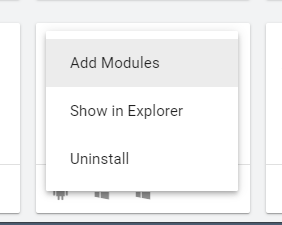
\includegraphics[width=0.6\textwidth]{img/hub3}
\caption{Se muestra la forma de acceder a la instalación de módulos.}
\end{figure}\label{fig13}
\imagen{hub2}{Se muestra la ventana para añadir los módulos.} 


\section{Compilación, instalación y ejecución del proyecto} \label{pepe}

Una vez instaladas todas las herramientas necesarias procederemos seguir los pasos para a la instalación y ejecución del proyecto. La generación de las \textit{buidls} se dividirá en 2 guías, una para cada aplicación.

El primer paso por realizar es abrir Unity Hub. Pulsamos en el botón \textit{add} y seleccionamos la carpeta principal del directorio del proyecto. Una vez seleccionado el proyecto nos aseguramos de seleccionar la versión de Unity correcta y abrimos el proyecto.

\imagen{unityhub}{Se muestra la ventana de Unity Hub donde seleccionamos la version correcta para iniciar el proyecto.}


\subsection{Ordenador}

Para configurar la aplicación del ordenador lo primero que debemos hacer es abrir su escena. Nos vamos la ventana de \textit{Project}, buscamos la carpeta \textit{Scenes} y hacemos doble clic sobre la escena con el nombre “video chat PC”.

\imagen{escenas}{Se muestra directorio del proyecto y la carpeta con las escenas}

Tras abrir la escena nos dirigiremos a la jerarquía de la escena y buscaremos el \textit{gameObject} con el nombre “Conexión”.

\imagen{jerarquiaordenador}{Se muestra jerarquía de la escena de la aplicación del ordenador.}

Haremos clic en el \textit{gameObject} y nos dirigiremos a la ventana del inspector. Ahí modificaremos el campo “http server addres” y lo cambiaremos por la \textit{IP} local de nuestro ordenador.

\imagen{2021-06-09 09_55_33-Window}{Se muestra la ventana de inspector del \textit{gameObject} “Conexión”.}

Por último, nos iremos a la ventana de \textit{File} y pulsaremos \textit{Build settings}. Ahí nos aseguraremos de que la escena cargada sea la del ordenador y que la plataforma utilizada para realizar la \textit{build} sea Pc, Mac \& Linux Standalone. Una vez realizadas las comprobaciones pulsaremos el botón de \textit{build} y elegiremos la carpeta de destino.

\begin{figure}
\centering
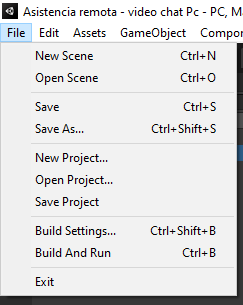
\includegraphics[width=0.3\textwidth]{img/buildsettings}
\caption{Se muestra la ventana de File y la opcion de \textit{build} settings.}
\end{figure}

\imagen{buildordenador}{Se muestra la ventana de para hacer \textit{builds} y toda su configuración}

Para ejecutar la aplicación simplemente deberemos dirigirnos a la carpeta de destino y ejecutaremos el fichero con la terminación .exe.

\subsection{HoloLens 2}

Comenzaremos abriendo la escena de “Hololens final” de la carpeta de \textit{Scene}. Nos dirigiremos a la jerarquía de la escena y buscaremos el textit{gameObject} con el nombre de “Conexión”.

\imagen{jerarquiahololens}{Se muestra jerarquía de la escena de la aplicación de las HoloLEns 2.}

Al igual que en la configuración de la aplicación del ordenador nos dirigiremos al la ventana del inspector y modificaremos el campo “http server addres” por la dirección \textit{IP} local de nuestro ordenador.

Posteriormente iremos a la ventana de \textit{Build settings} y esta vez seleccionaremos la opción de “Windows Universal Platform”. Pulsaremos el botón de \textit{Switch platform}. Una vez finalice los cambios borraremos la escena de la aplicación del ordenador y pulsaremos el botón de \textit{Add open scenes}.

\imagen{switch}{Se muestra la ventana de para hacer \textit{builds} sin haber cambiado de plataforma.}

Sin modificar ningún de valor de la configuración pulsaremos el botón de \textit{build} y seleccionaremos la carpeta de destino.

\imagen{buildhololens}{Se muestra la ventana de para hacer \textit{builds} después de cambiar la plataforma y la escena.}

Nos dirigiremos al directorio de destino y ejecutaremos con Visual Studio 2019 el archivo “Asistencia Remota.sln”

\imagen{visual}{Se muestra el directorio con la \textit{build}}

Seleccionamos el desplegable de “Máquina remota” y hacemos clic en el apartado de propiedades.

\imagen{configuracion}{Se muestra el desplegable con las diferentes opciones de compilación.}

Vamos a “Propiedades de depuración” -> “Depuracion” -> “Nombre del equipo” y modificamos el valor con la dirección \textit{IP} local de las Hololens 2.
\imagen{configuracion2}{Se muestra la ventana con las propiedades de la depuración.}

Por último, nos aseguramos de que estén seleccionadas las opciones de “Master” y “ARM” y pulsamos el botón verde del \textit{play}.

\imagen{instalacion}{Se muestra las opciones de depuración.}


\apendice{Documentación de usuario}

\section{Introducción}

Como el resultado del proyecto son dos aplicaciones distintas, la documentación de usuario se encontrará fraccionada en dos partes: una para el técnico que utilice la aplicación desde el ordenador y otra para el usuario sin formación que utiliza las HoloLens 2.

\section{Requisitos de usuarios}

Para el uso del resultado de este proyecto de necesitarán dos componentes hardware imprescindibles, un ordenador y unas HoloLens 2.

Las especificaciones del ordenador serán las mismas que las expuestas en el manual de programador~\ref{recomendados}, es decir, los requisitos recomendaos para usar el software de Unity.

\begin{table}[ht!]
\centering
\begin{tabular}{|l|p{0.8\linewidth}|}
\hline
\multicolumn{2}{|l|}{\cellcolor[HTML]{C0C0C0}Requisitos recomendados.}                                                           \\ \hline
Sistema Opererativo         & Windows 7 / 8 / 10                                                                                                                                               \\ \hline
Procesador           & Core 4 Duo ó superior    \\ \hline
Memoria     & \begin{tabular}[c]{@{}p{\linewidth}@{}} 2 GB de RAM \end{tabular} \\ \hline
Gráficos  & DirectX11 Compatible GPU con 1 GB Video RAM   \\ \hline
Almacenamiento        &  100 MB de espacio disponible   \\ \hline
Tarjeta de sonido & \begin{tabular}[c]{@{}p{\linewidth}@{}} DirectX compatible Tarjeta de sonido\end{tabular}    \\ \hline
\end{tabular}
\caption{Se muestran los requisitos recomendados por Unity para su software.}
\end{table}

Para complementar el ordenador se necesitará una \textit{webcam} y unos auriculares con micrófono para poder entablar una conversación con el usuario de las HoloLens 2.

Para poder usar la otra parte del proyecto solamente se necesitarán las HoloLens 2, ya que estas están provistas del todo el hardware necesario para aprovechar todas las funcionalidades de la videoconferencia.

\section{Instalación}

Para instalar las aplicaciones en ambos dispositivos se seguirán los mismos pasos ya explicados en el apartado de compilación, instalación y ejecución del proyecto~\ref{pepe} en el manual del programador. 

Importante tener ejecutado el servidor de Node.js cada vez que se quiera utilizar las aplicaciones.

\imagen{nodeconexion}{Se muestra la ejecución del proyecto node-dss con ambos dispositivos conectados.}

\section{Manual del usuario}

\subsection{HoloLens 2}

Antes de ponernos las gafas deberemos conocer la utilidad de los botones físicos con los que cuenta. Las funcionalidades son las siguientes:
\begin{enumerate}
    \item \textbf{Botón de encendido/apagado: }Pulsaremos rápidamente el botón para encender las gafas y mantendremos pulsado unos 3 segundos aproximadamente para apagarlas. 
    \item \textbf{Puerto de carga: }A través de este puerto repondremos la batería de las gafas cuando sea necesario. El extremo del cable que conectemos a las gafas debe ser tipo USB-C.
    \item \textbf{Botón de subir/bajar volumen: }El volumen tiene un valor mínimo de 0 y un máximo de 100. Sumaremos o restaremos 10 a este valor pulsando parte del botón donde pone + o - respectivamente.
    \item \textbf{Botón de subir/bajar brillo: }Al igual que el volumen este tiene un valor mínimo de 0 y un máximo de 100. También sumaremos o restaremos 10 a este valor pulsando parte del botón donde pone + o - respectivamente.
\end{enumerate}



\imagen{holo2}{Se muestra un lateral de las HoloLens 2 donde se encuentran los botones de encendido, volumen, y la ranura de carga.}
\imagen{holo3}{Se muestra un lateral de las HoloLens 2 donde se encuentran el botón del brillo.}

Una vez conocidas las funciones de los botones de las gafas nos las pondremos en la cabeza y pulsaremos el botón de encendido. Tras cargar el sistema operativo tendremos que poner el código PIN elegido previamente por nosotros durante el primer uso del dispositivo de realidad mixta.

Después de poner el código correctamente, tendremos que mirar la muñeca de nuestra mano hasta que aparezca el logo de Windows y pulsarlo con el dedo (véase Fig E.4 sección \ref{fig9}). 

\imagen{mano}{Se muestra como abrir el menú principal de las HoloLens 2.\label{fig9}}

A continuación, tras abrir el menú, pulsamos con el dedo la opción a la derecha llamada “todas”, que mostrará un listado de todas aplicaciones instaladas en las gafas. En ese listado buscaremos la aplicación llamada asistencia remota y la pulsaremos. 

\imagen{menu1}{Se muestra el menú inicial de las HoloLens 2.}
\imagen{menu2}{Se muestra la ventana con todas las aplicaciones instaladas.}

Una vez abierta la aplicación proporcionaremos el código al usuario que esté en la aplicación del ordenador y esperaremos a que se establezca la conexión.

\imagen{codigo}{Se muestra la ventana inicial de la aplicación donde obtenemos el código.}

Tras establecer la conexión se nos mostrará una interfaz y una pantalla en realidad virtual. Las funcionalidades de la interfaz son las siguientes:

\begin{enumerate}
    \item \textbf{Pantalla:} Pantalla en realidad aumentada donde visualizaremos la imagen recibida de la \textit{webcam} del ordenador. Se puede mover, aumentar o disminuir de tamaño, rotar...
    \item \textbf{Barra de menú:} Barra de menú que contiene todos los botones. Se puede mover, aumentar o disminuir de tamaño, rotar...
    \item \textbf{Botón de silenciar:} Botón que silencia el micrófono de las HoloLens 2.
    \item \textbf{Botón de esconder \textit{webcam}:} Botón que esconde la pantalla en realidad aumentada.
    \item \textbf{Botón de ensordecer:} Botón que elimina el sonido de toda la aplicación.
    \item \textbf{Botón de finalizar la llamada:} Botón que finaliza la llamada.
    \item \textbf{Botón de activar/desactivar el seguimiento radial de la interfaz:} Botón que activa o desactiva el seguimiento de la interfaz sobre el movimiento de nuestra cabeza.
    \item \textbf{Botón de esconder/mostrar la interfaz:} Botón que esconde o vuelve a activar la interfaz en realidad aumentada.
\end{enumerate}

\imagen{vistahololens}{Se muestra la pantalla virtual donde se retransmite la \textit{webcam} del ordenador y la interfaz con sus botones en realidad aumentada.}
\newpage
\subsection{Ordenador}
Primero ejecutaremos el archivo de extensión \textit{.exe} creado tras hacer la \textit{build} del proyecto. Una vez abierta la pantalla de inicio colocaremos el código proporcionado por el usuario con las HoloLens 2 y pulsaremos el botón verde para iniciar la videollamada.

\imagen{itroducircodigo2}{Se muestra la ventana inicial de la aplicación del ordenador.}

En esta ventana se observará la retransmisión de la perspectiva de las HoloLens 2, una interfaz y nuestra propia \textit{webcam}: 
\begin{enumerate}
    \item \textbf{Pantalla:} Pantalla que muestra la vista de las gafas.
    \item \textbf{\textit{Webcam}:} En la esquina inferior derecha se mostrará nuestra \textit{webcam} si la tenemos conectada.
    \item \textbf{Botón de generar indicadores:} Botón que tras hacer clic en la pantalla, generará una flecha en realidad aumentada en el punto del espacio correspondiente.
    \item \textbf{Botón de deshacer:} Botón que elimina el ultimo indicador generado.
    \item \textbf{Botón de borrar:} Botón que elimina todos los indicadores de la escena.
    \item \textbf{Botón de silenciar:} Botón que silencia el micrófono.
    \item \textbf{Botón de desactivar la \textit{webcam}:} Botón que desactiva la \textit{webcam}.
    \item \textbf{Botón de finalizar la llamada:} Botón que finaliza la llamada.
\end{enumerate}

\imagen{vistaordenador}{Se muestra la retransmisión de la perspectiva de las HoloLens 2 en el ordenador y nuestra propia \textit{webcam}.}



\bibliographystyle{plain}
\bibliography{bibliografiaAnexos}

\end{document}
